\chapter{Metodologia}

Para estudar a influência do sono na formação e recordação de conjuntos celulares será simulado um modelo de RND com diferentes
formas de plasticidade.

\section{Modelo da rede neural de disparos}

A rede será composta de 5120 neurônios LIF, sendo 4096 excitatórios e 1024 inibitórios. Cada neurônio da rede será conectado a de
forma aleatória a 10\% dos neurônios da rede. Todas as conexões sinápticas serão implementadas com modelos de plasticidade. Além
disso, a rede será conectada a uma ``retina'' simulada, que receberá os estímulos de imagem em uma resolução de 64$\times$64
pixels; cada neurônio da rede receberá conexões de uma área circular de alguns neurônios da retina.

\section{Estímulos}

Os estímulos serão imagens simples de serem reconhecidas, como formas geométricas e símbolos. Os estímulos serão apresentados à
rede de forma intercalada e aleatória, também haverão momentos da simulação em que nenhum estímulo será apresentado. Nesse último
caso, cada neurônio da retina vai se comportar com uma unidade de Poisson que dispara de forma aleatória.

\section{Simulação do sono}

Para simular o sono, a rede funcionará de dois modos diferentes intercalados: um modo de atividade, em que a rede vai funcionar
normalmente enquanto recebe estímulos, e um modo de inatividade, em que será simulado o sono. 

Durante a fase de inatividade, nenhum estímulo será apresentado à rede, mas ela vai continuar sendo simulada normalmente. Além
disso, essa fase será dividida em subfases de acordo com as fases do sono real. Para simular cada fase do sono, os neurônios
receberão uma corrente sinusoidal de frequência e amplitude diferentes para cada fase de modo a tentar imitar os padrões de
atividade cerebral durante o sono observados em eletroencefalograma; também serão simulados outros sinais característicos do sono
de forma similar injetando corrente, como os fusos do sono que ocorrem durante a fase N2.

\section{Detalhes da simulação}

Todo o código da simulação será escrito em C++ utilizando o framework Auryn~\cite{zenkeLimits2014}.

\section{Análise}

Para determinar quais neurônios pertencem ao conjunto celular associado a um estímulo, será analisada a frequência de disparos de
cada neurônio no intervalo $3s < t < 3.5s$ após a apresentação do estímulo. Os neurônios que dispararem com frequência maior que
10Hz serão considerados como pertencentes ao conjunto celular associado ao estímulo.


\section{Cronograma}

\begin{table}[!ht]
\Caption{Cronograma de atividades.}
\centering\label{fig_cronograma}
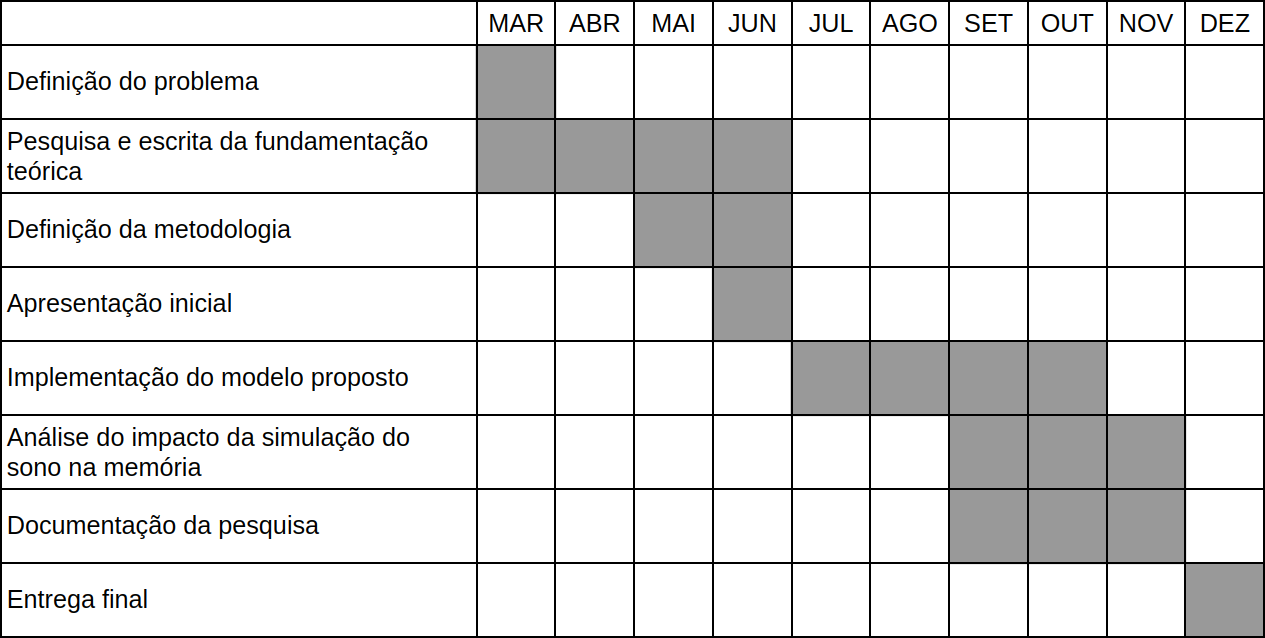
\includegraphics[width=\linewidth]{figuras/cronograma.png}
% \Fonte{}
\end{table}